\chapter{Reconstrucción e identificación de objectos físicos} %
% \addcontentsline{toc}{chapter}{Reconstrucción e identificación de objectos físicos}
\chaptermark{Reconstrucción e identificación de objectos físicos}



El diseño del detector ATLAS permite la reconstrucción e identificación de prácticamente todas las
partículas producidas en la colisión $pp$. 
La mayoría de las partículas del SM son inestables por lo que decaen rápidamente en otras partículas estables. Esto reduce considerablemente las posibles partículas que llegan
al detector, ya que solo van a ser aquellas que sean estables o vida media suficientemente larga, siendo estas principalmente: $\gamma$, $e^{\pm}$, $\mu^{\pm}$, $\nu$ y algunos hadrones
como $p$, $n$, piones y kaones. El diseño de los distintos subdetectores permite aprovechar las
características de cada una de ellas, haciendo que cada una de las partículas anteriores depositen señales distintivas, permitiendo su reconstrucción e identificación. La Figura \ref{particulasATLAS} muestra un esquema de las distintas señales producidas por cada una de las partículas en el detector ATLAS. Todos los procesos de reconstrucción descriptos a continuación se realizan sobre los datos que fueron almacenados en disco (\textit{offline}), a partir de eventos que pasaron los requisitos del sistema de trigger y almacenamiento durante lo toma de datos (\textit{online}).


% / Reescrito /
% Dada la energía de colisión entregada por el LHC, es
% posible producir todas las partículas del SM. Las partículas que tienen una vida media muy corta,
% decaen antes de llegar a la parte más interna del detector y se detectan los productos de su
% decaimiento. Teniendo en cuenta esto, se reduce considerablemente las posibles partículas que llegan
% al detector, ya que solo van a ser aquellas que sean estables o con suficiente vida media. Estas
% partículas consisten prácticamente en: $\gamma$, $e^{\pm}$, $\mu^{\pm}$, $\nu$ y algunos hadrones
% como $p$, $n$, piones y kaones. El diseño de los distintos subdetector permite aprovechar las
% características de cada una de ellas, permitiendo su reconstrucción e identificación. La
% reconstrucción se realiza una vez que el evento pasó los requisitos del \trigger y fue almacenado
% (\textit{offline}) \tosolve{Revisar todo este párrafo}


\begin{figure}
\centering
  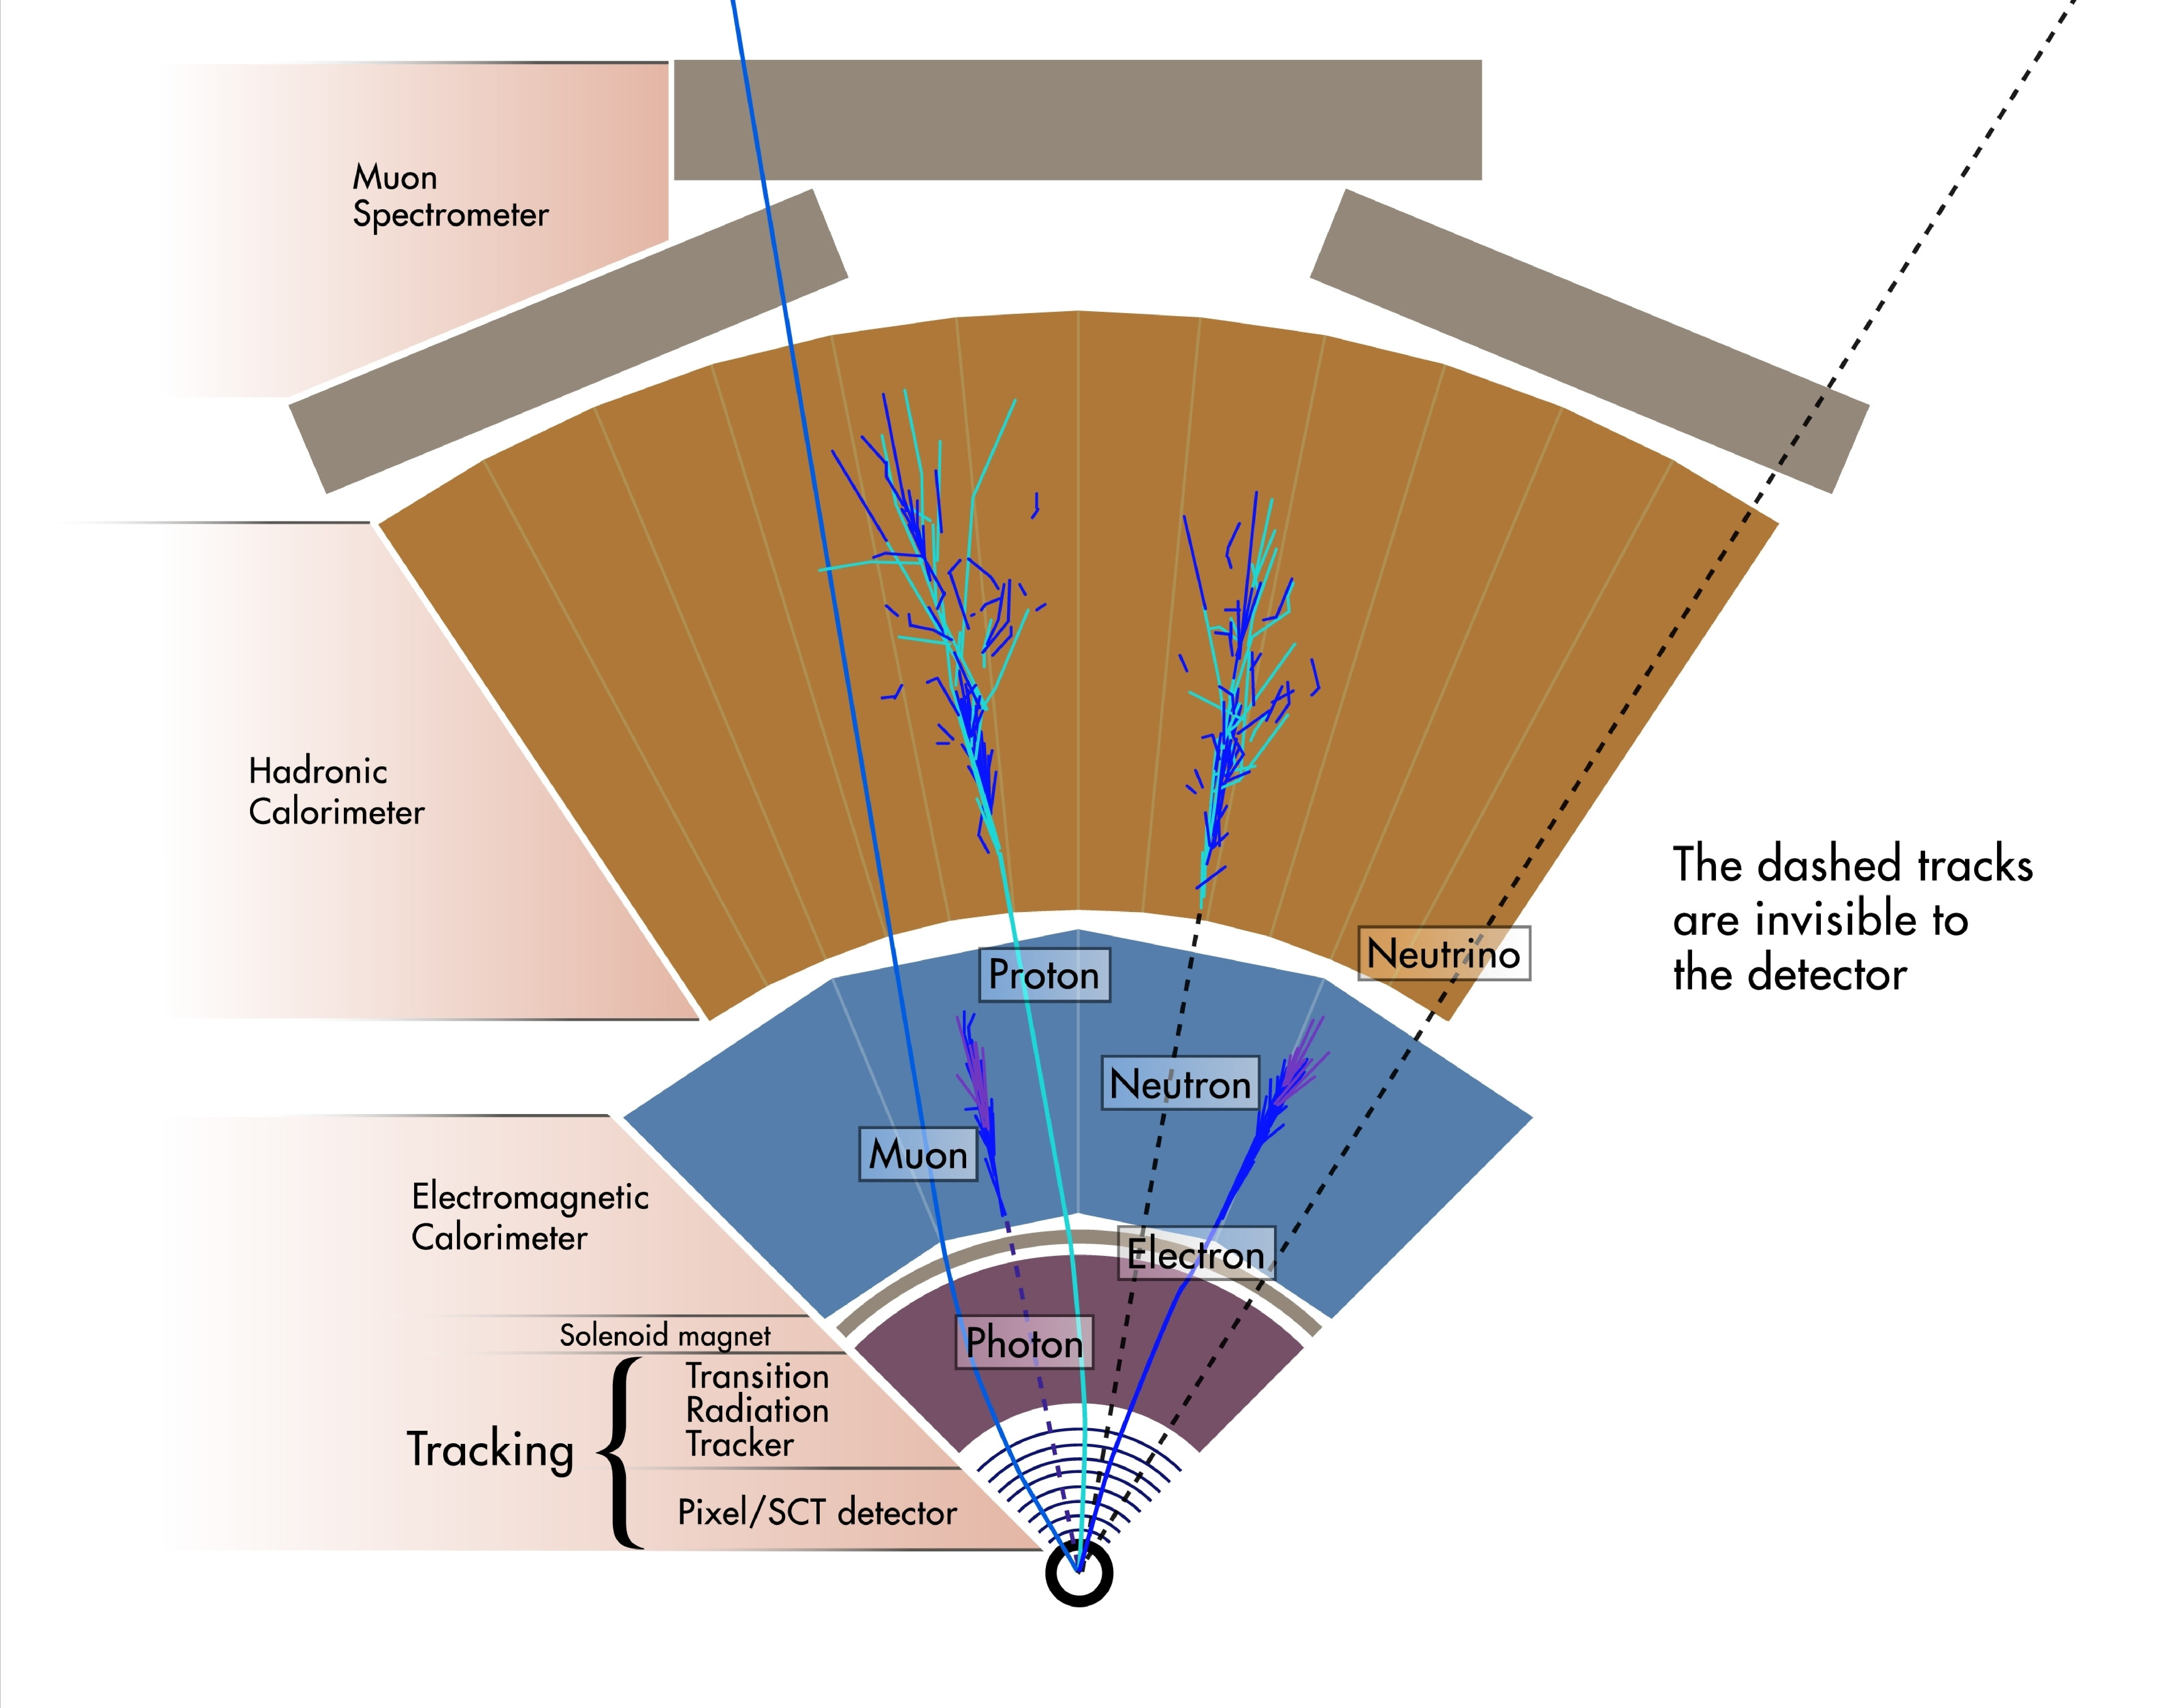
\includegraphics[width=0.6\textwidth]{images/cross_section_2-eps-converted-to.pdf}
\caption{Esquema de los distintos tipos de señal que pueden dejar las partículas en el detector ATLAS. \tosolve{Mejorar imagen} 
% \commentyellow{Puede omitirse esta imagen} 
% \commentNotaIII 
}
\label{particulasATLAS}
\end{figure}

\section{Electrones y fotones}\label{sec:ph_el}

% / Reescrito /
% La reconstrucción de electrones y fotones en el detector ATLAS se realiza principalmente a partir de los depósitos
% de energía medidos en el calorímetro electromagnético. Como la deposición de ambas partículas son
% similares, se utiliza además información del detector de trazas para poder distinguir una de otra.
% Las técnicas de reconstrucción de electrones y fotones son similares y por ende pueden ser
% descriptas simultáneamente.

Los electrones y fotones producidos tanto en la colisión $pp$ como aquellos producto del decaimiento de otras partículas, depositan la mayor parte de su energía en el ECAL. Estos depósitos están restringidos a un número de celdas vecinas cuyo conjunto se denomina \textit{cluster}, y que tienen estructuras propias de estas partículas. Los depósitos que dejan ambas partículas son similares y con el objetivo de poder distinguirlas se utiliza además información del detector de trazas. Al ser el fotón una partícula neutra no deja traza en el ID, por lo que los clusters que no están asociados a trazas son considerados fotones, mientras que los que los que sí lo están son considerados electrones. 

Procesos como la producción de pares ($\gamma\to e^{-}e^{+}$) producto de la interacción de los fotones con el material del detector, pueden dejar trazas o depósitos que no corresponden con la reconstrucción de un fotón. El algoritmo de reconstrucción tiene en cuenta esto y puede reconstruir los vértices de conversión, por lo que los clusters asociados a vértices de conversión son considerados fotones. Finalmente, ciertos procesos (ej. $\pi^{0}\to\gamma\gamma$) pueden generar depósitos que erróneamente son reconstruidos como fotones o electrones
\tosolve{Tenía una duda sobre la identificación de los pi0}
. Para reducir la identificación errónea se aplican entonces una serie de criterios de identificación y aislamiento, basados en las formas de los depósitos de energía, que permiten discriminar estos procesos de los procesos prompt.
\tosolve{Habria que definir prompt, pero surgieron dudas sobre la definición de prompt object que estaría bueno solucionar.}
% \commentyellow{Ver dudas sobre la definicion de prompt}
Las técnicas de reconstrucción de electrones y fotones son similares, y se realizan de forma simultánea.

\subsection{Reconstrucción}


La reconstrucción de electrones y fotones en el detector ATLAS se realiza utilizando un algoritmo para la reconstrucción de clusters dinámicos de tamaño variable, denominados \textit{topo-clusters} que se agrupan además en \textit{superclusters}\cite{EGAM-2018-01}. Durante Run 1 el algoritmo reconstruía clusters de tamaño fijo \cite{PERF-2013-04, PERF-2013-05, Lampl:1099735}, que si bien tenían una respuesta lineal energética y un estabilidad frente a pile-up, no permitía reconstruir eficientemente la energía de fotones \textit{bremsstrahlung} o de electrones/positrones producto de la creación de pares. La implementación de superclusters durante el Run 2, junto con la calibración de la energía descripta en la Referencia \cite{PERF-2017-03} permite solucionar esto sin perder la linealidad y estabilidad de los clusters de tamaño fijo.

\subsubsection{Topo-clusters}

El algoritmo comienza buscando las celdas en el ECAL y el HCAL con una señal\footnote{Para los topo-clusters electromagnéticos la medida de la señal se realiza en la escala electromagnética, que es la escala adecuada para medir los depósitos de energía de las partículas producidas en lluvias electromagnéticas de forma correcta} cuatro veces mayor al ruido esperado dadas las condiciones de luminosidad y pileup del Run 2. A partir de ellas agrega las celdas vecinas cuya señal sea dos veces mayor al ruido
% \commentHW{esta definido ruido ? hace falta ahcerlo aca ?}
% \commentgreen{No sé que tanto debería definir ruido, en la línea anterior indica que es el ruido esperado dadas las condiciones... Habrá que aclarar algo más? Puede que en esta línea suene medio vago y tenga que agregar algo}
, que a su vez son utilizadas en la siguiente iteración del algoritmo, que se repite hasta que no haya más celdas adyacentes que cumplan este requisito. Finalmente se agregan todas las celdas vecinas a las celdas anteriores, independientemente de la intensidad de señal que tengan, formando lo que se denominan topo-clusters \cite{PERF-2014-07, Lampl:1099735}. Los topo-clusters que compartan celdas son unificados, mientras que los topo-clusters que tengan dos máximos locales son divididos.

\tosolve{Preguntar: Electron and photon reconstruction starts from the topo-clusters but only uses the energy from cells in the EM calorimeter,  This is referred to as theEM energy of the cluster, and the EM fraction (fEM) is the ratio of the EM energy to the total cluster energy. No usa la parte del HCAL?}

\subsubsection{Trazas y vértices de conversión}

La reconstrucción de trazas se realiza utilizando un algoritmo de búsqueda de patrones de trazas estándar
% \commentHW{decir algo más que estándar ?}
% \commentgreen{En realidad lo traduje de `Standard track-pattern reconstruction', puede que haya que mejorarlo}
\cite{newt, PERF-2017-02, PERF-2017-01} en todo el ID. A su vez, utiliza los depósitos en el ECAL que presenten una forma compatible con la de una lluvia electromagnética para definir regiones de interés. En caso de que el algoritmo anterior falle, se utiliza en estas regiones otro algoritmo de búsqueda de trazas \cite{Kalman}, permitiendo reconstruir trazas adicionales. Luego se realiza una serie de ajustes ($\chi^2$ \cite{chi2}, GSF \cite{gsf}) de las trazas permitiendo obtener correctamente los parámetros que la caracterizan. Finalmente las trazas son asociadas a los topo-clusters extrapolando a la misma desde el perigeo hasta la segunda capa del ECAL. Una traza se considera asociada con un topo-clusters si $|\eta_{\text{traza}}-\eta_{\text{cluster}}|<0.05$ y $-0.10<q\cdot(\phi_{\text{traza}}-\phi_{\text{cluster}})<0.05$, donde $q$ es la carga de la traza. A su vez, el momento de la traza es escaleado para que coincida con al energía del topo-cluster asociado. Si múltiples trazas son asociadas a un mismo topo-cluster se clasifica a las mismas utilizando criterios de calidad, siendo la mejor clasificada la que se utiliza para reconstruir a los electrones. 

Los vértices de conversión son reconstruidos a partir de pares de trazas con cargas de signo opuesto y consistentes con el decaimiento de una partícula sin masa. Adicionalmente se pueden reconstruir vértices de conversión a partir de una sola traza que no haya dejado señal en las capas más internas del ID. En ambos casos se busca que la traza tenga altas probabilidad de ser un electrón en el TRT \cite{trt} pero baja en el SCT. Es esperado que las trazas de los vértices de conversión estén muy cerca una de otra, en general compartiendo \textit{hits}, haciendo que una de las trazas no llegue a reconstruirse. Para ello se utilizan trazas con requisitos de asociación a topo-clusters más relajados que los anteriormente descriptos, y con distintos criterios de ambigüedad ante solapamiento. Finalmente los vértices son asociados a los topo-clusters, y en caso de múltiples vértices asociados a un mismo topo-cluster se prioriza aquellos reconstruidos a partir de dos trazas y cuyo radio sea menor.

\subsubsection{Superclusters}

La reconstrucción de los superclusters para electrones y fotones se realiza de forma independiente y en dos etapas: primero se encuentran los topo-clusters semilla 
% \commentyellow{Capaz pueda modificar el texto para que la palabra semilla quede mejor}
 y luego se le adjuntan los topo-clusters satélites producidos generalmente por \textit{bremsstrahlung} o por la división de topo-clusters. El algoritmo comienza ordenando todos los topo-clusters por \ET y verifica si pasan los requerimientos para ser un topo-clusters semilla (comenzando por los más energéticos). En el caso de los electrones el requisito es tener \ET mayor a $1$ GeV y una traza asociada con al menos cuatro \textit{hits} en el SCT, mientras que el de los fotones es tener \ET mayor a $1.5$ GeV. Cuando un topo-clusters pasa estos requisitos se busca sus topo-clusters satélites asociados y el mismo no puede ser utilizado como satélite en las siguientes iteraciones. Los topo-clusters satélites son aquellos que se encuentran dentro de una ventana de $\Delta\eta\times\Delta\phi=0.075\times0.125$ alrededor del centro del topo-cluster inicial. Para electrones además se consideran topo-clusters satélites aquellos que se encuentran dentro de una ventana de $\Delta\eta\times\Delta\phi=0.125\times0.3$ cuya traza mejor ajustada coincide con la traza mejor ajustada del topo-cluster inicial. Para fotones convertidos además se consideran topo-clusters satélites aquellos que compartan el vértice de conversión con el topo-cluster inicial. 

Para limitar la sensibilidad de los superclusters al pileup, el tamaño de cada topo-cluster constituyente es restringido a un máximo de $0.075$ ($0.125$) en la dirección de $\eta$  en la región barrel (endcap). Como el algoritmo se utiliza de forma independiente tanto para electrones como para fotones, puede ocurrir que un mismo supercluster se asocie tanto a un electrón como a un fotón. En ese caso se utilizan una serie de criterios de ambigüedad que permiten determinar si el candidato es un electrón o un fotón. En el caso que aún no pasen los criterios de ambigüedad el candidato es guardado como electrón y fotón simultáneamente, pero marcados como ambiguos y es decisión de cada análisis incluirlos en el mismo.
% \commentyellow{posible pie para hablar del overlap removal OR?}

Finalmente se calibra la energía de los superclusters, las trazas son nuevamente ajustadas pero ahora utilizando los superclusters anteriores, y la energía es recalibrada teniendo en cuenta este nuevo último ajuste siguiendo el procedimiento descripto en la Referencia \cite{PERF-2017-03}.

% / Reescrito /
% A continuación el algoritmo construye los superclusters para electrones y fotones por separado. Para ello selecciona los topo-clusters con una energía mayor a cierto \tosolve{Nota 1} umbral, y los agrupa con los demás topo-clusters satélites que estén contenidos dentro de una ventana angular fija centrada en el \textit{topo-cluster} inicial. Dependiendo si el algoritmo es para fotones o electrones los umbrales son distintos, y en el caso de electrones o fotones convertidos, topo-clusters satélites adicionales son incluidos utilizando las trazas asociadas. Como los \textit{supercluster} de electrones y fotones son generados independientemente, puede ocurrir que un mismo \textit{supercluster} produzca tanto un electrón como un fotón. En ese caso el candidato es guardado tanto como electrón y fotón simultáneamente, pero marcados como ambiguos y es decisión de cada análisis utilizarlos o no. Al finalizar esta etapa se obtienen los objetos finales que van a ser utilizados por los distintos análisis. \tosolve{calibración? eficiencia?}

\subsection{Identificación}\label{sec:ph_id}

Como se mencionó anteriormente, distintos criterios de identificación son utilizados para poder discriminar los objetos prompt
% \commentyellow{Ver dudas sobre la definicion de prompt} 
de aquellos que no lo son. Para ello se definen una serie de variables basadas en la información del calorímetro y del ID, que mediante distintas técnicas permiten la correcta identificación de los objetos. Finalmente se definen diferentes puntos de trabajo (\textit{Working Points}, WP) que permiten mejorar la pureza de los objetos seleccionados al costo de tener una menor eficiencia de selección.

La identificación de electrones tiene como principal objetivo discriminar los electrones prompt de los fotones convertidos, de jets que depositaron energía en el ECAL y de electrones producidos en el decaimiento de hadrones de sabor pesado. Esta identificación se basa en un método de likelihood que utiliza algunas de las variables descriptas en la Tabla \ref{phIDVars}, y cuyas PDFs se obtienen de eventos con decaimientos de $J/\Psi$ y $Z$ para electrones de bajo y alto \ET respectivamente \cite{PERF-2016-01}. Para electrones se definen tres WP, \texttt{Loose}, \texttt{Medium} y \texttt{Tight}, cuyas eficiencias de identificación promedio son  93\%, 88\% y 80\% respectivamente.

La identificación de fotones esta diseñada para seleccionar eficientemente fotones prompt. y rechazar los fotones falsos provenientes de jets, principalmente del decaimiento de mesones livianos ($\pi^{0}\to\gamma\gamma$). La identificación se basa en una serie de cortes rectangulares sobre las variables presentes en la Tabla \ref{phIDVars}. Las variables que utilizan las primeras capas del ECAL son esenciales para discriminar los decaimientos del $\pi^{0}$ en dos fotones muy colimados, ya que los depósitos de energía de este decaimiento se extienden en más celdas de este capa en comparación con el depósito de un fotón real. En la Figura \ref{phpizero} se puede observar la comparación de ambos procesos. 
Para la identificación de fotones también se definen tres WPs, \texttt{Loose}, \texttt{Medium} (empleado solamente en la reconstrucción en el HLT) y \texttt{Tight}, cada uno inclusivo con respecto al anterior, y en la Tabla \ref{phIDVars} se muestran las variables empleadas por cada uno de ellos. 
% Los WPs \textit{Loose} y \textit{Medium} fueron utilizados por los algoritmos del trigger durante la toma de datos del Run 2 para seleccionar eventos con uno o dos fotones. 
Como los depósitos de energía varían debido a la geometría del calorímetros, los tres WPs fueron optimizados para diferentes valores de $|\eta|$, y adicionalmente la selección \texttt{Tight} fue optimizada para distintos valores de \ET. Los depósitos de energía de los fotones convertidos difiere de los no convertidos, debido a la separación angular entre el $e^-$ y el $e^+$ que se amplifica por el campo magnético, y debido a la interacción de los pares con capas más altas del calorímetro, permitiendo optimizar la selección \texttt{Tight} de forma separada para fotones convertidos de los no convertidos. Esto no fue posible para las selecciones \texttt{Loose} y \texttt{Medium} ya que la información que utilizan no permite saber si un fotón es convertido o no. La optimización fue realizada a bajo \ET utilizando simulaciones de decaimientos radiativos del bosón $Z$ junto con datos con eventos con bosones $Z$, y a alto \ET con simulaciones de producción de fotones inclusiva y jets. La eficiencia de identificación para la selección \texttt{Tight} supera el 80\% para fotones con $\ET>20$ GeV \cite{EGAM-2018-01}.

\begin{figure}
  \centering
  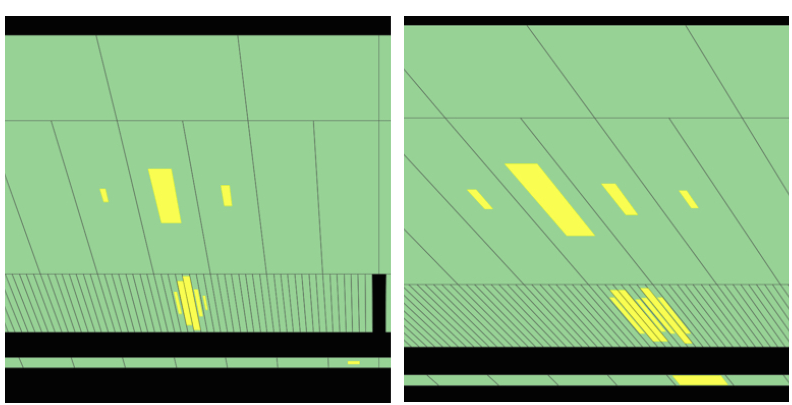
\includegraphics[width=0.7\textwidth]{images/PhotonPizero.png}
  \caption{Depósitos de energía característicos de un fotón aislado (izquierda) y un $\pi^0$ (derecha).
  \tosolve{Seguro haya una imagen de mejor calidad} 
  }
  \label{phpizero}
\end{figure}


\begin{table}
\centering 
\caption{Variables utilizadas en la definición de los WPs de identificación de fotones, \texttt{Loose} (L), \texttt{Medium} (M) y \texttt{Tight} (T). La identificación de electrones utiliza, además de algunas de estas, variables adicionales que no se muestran en la tabla. Para las variables de la primer capa del ECAL, si el cluster tiene más de una celda en la dirección de $\phi$ a un dado $\eta$, las dos celdas más cercanas en $\phi$ al baricentro del cluster son combinadas y las variables se consideran utilizando esa celda combinada. \tosolve{Algunas definiciones no son muy claras, tampoco en el paper...}}
	\begin{tabular}{ l p{2cm} p{8cm} c c c}

		Categoría & Nombre & Descripción & L & M & T \\

		\hline
		\hline

		Fuga hadrónica & $R_{\text{had}_{1}}$ & Fracción de \ET en la primer capa del HCAL con respecto al \ET total del cluster (para $|\eta|<0.8$ y $|\eta|>1.37$) & \cmark & \cmark & \cmark\\

		 & $R_{\text{had}}$ & Fracción de \ET en el HCAL con respecto al \ET total del cluster (para $0.8<|\eta|<1.37$) & \cmark & \cmark & \cmark \\

		\hline
		
		$2^{\text{da}}$ capa del ECAL  & $w_{\eta 2}$ & Ancho lateral de la lluvia: $\sqrt{\frac{\Sigma E_{i}\eta_{i}^{2}}{\Sigma E_{i}}-(\frac{\Sigma E_{i}\eta_{i}}{\Sigma E_{i}})^{2}}$, donde la suma es calculada en una ventana de $3\times5$ celdas & \cmark & \cmark & \cmark \\

		 & $R_{\eta}$ & Fracción de la suma de las energías contenida en un rectángulo de $\eta\times\phi = 3\times7$ celdas con respecto a un rectángulo $7\times7$ celdas, ambos centrados en la celda más energética & \cmark & \cmark & \cmark \\

		 & $R_{\phi}$ & Fracción de la suma de las energías contenida en un rectángulo de $\eta\times\phi = 3\times3$ celdas con respecto a un rectángulo $3\times7$ celdas, ambos centrados en la celda más energética & \xmark & \xmark & \cmark \\

		\hline


		$1^{\text{er}}$ capa del ECAL & $E_{\text{ratio}}$ & Fracción entre la diferencia de energías del máximo depósito y el segundo, y la suma de ambos & \xmark & \cmark & \cmark \\

		 & $w_{s\:\text{tot}}$ & Ancho lateral total de la lluvia: $\sqrt{\frac{\Sigma E_{i}(i-i_{\text{máx}})^{2}}{\Sigma E_{i}}}$, donde la suma se realiza sobre todas las celdas contenidas en una ventana de $\Delta\eta\approx0.0625$ e $i_{\text{máx}}$ es la celda con mayor energía & \xmark & \xmark & \cmark \\

		 & $w_{s\:\text{3}}$ & Ancho lateral de la lluvia: $\sqrt{\frac{\Sigma E_{i}(i-i_{\text{máx}})^{2}}{\Sigma E_{i}}}$, donde la suma se realiza sobre todas las celdas contenidas en una ventana de tres celdas alrededor de la celda de mayor energía, $i_{\text{máx}}$ & \xmark & \xmark & \cmark \\

		 & $f_{\text{side}}$ & Fracción de energía fuera de un núcleo con tres celdas centrales y dentro de siete celdas & \xmark & \xmark & \cmark \\

		 & $\Delta E_{s}$ & Diferencia entre la energía de la celda asociada con el segundo máximo, y la energía reconstruida en la celda con el valor menor entre el primer y segundo máximo & \xmark & \xmark & \cmark \\

		 & $f_{\text{1}}$ & Fracción de energía medida en la primer capa del ECAL con respecto a la energía total del cluster electromagnético & \xmark & \xmark & \cmark \\




	\end{tabular}

\label{phIDVars}
\end{table}




\subsection{Aislamiento}
\label{isolation}


Criterios de aislamiento se pueden aplicar sobre los fotones y electrones para aumentar aún más calidad de selección de los mismos. A su vez, la presencia de otros objetos cerca del fotón o el electrón puede interferir en la correcta reconstrucción de las variables cinemáticas del mismo, como su energía. El aislamiento de estos objetos se puede cuantizar definiendo variables no solo para los depósitos de energía, sino también para las trazas.

La variable de aislamiento calorimétrico \cite{PERF-2017-01} (\ETcone{X}) se define entonces como la suma de la energía transversa de todas las celdas contenidas en un cono centrado en el topo-cluster, y cuyo radio $\Delta R$ \footnote{$\Delta R=\sqrt{\Delta\phi^2+\Delta\eta^2}$} (en el plano $\eta-\phi$) es igual a X/100. La contribución energética del objeto a asilar se sustrae ignorando las celdas contenidas en un rectángulo en el centro del cono, y cuyos lados miden $\Delta\eta\times\Delta\phi = 5 \times 7$ como muestra la Figura \ref{IDcone}. Las filtraciones energéticas del candidato fuera del rectángulo son tenidas en cuenta junto con los efectos de pileup \cite{Cacciari}. Para electrones se utiliza un cono de radio $\Delta R = 0.2$ (\ETcone{20}), mientras que para fotones se utiliza uno de $\Delta R = 0.2$ (\ETcone{20}) o $\Delta R = 0.4$ (\ETcone{40}) dependiendo del WP.


\begin{figure}
\centering
  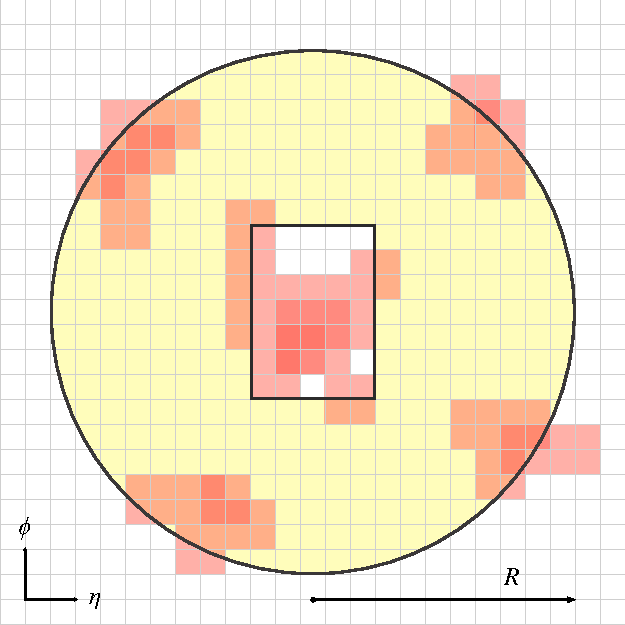
\includegraphics[width=0.4\textwidth]{images/iso.pdf}
\caption{Esquema del cono utilizado para el cálculo de la variable de aislamiento calorimétrico. 
% \commentNotaIII 
}
  \label{IDcone}
\end{figure}


% \commentHW{Agregar algún nexo con el párrafo anterior. Le falta algo de continuidad al texto. Algo como Otro segundo criterio de aislamiento complementario se define en base a la trazas reconstruidas de los objetos...}
% \commentgreen{Lo había pensado así: en el primer parrafo indico que hay 2 tipos de aislamiento, y después le dedico un párrafo no muy extenso a cada uno. Modifiqué un poco para que tenga algo más de continuidad}
La segunda variable de aislamiento se obtiene en base a las trazas de los objetos reconstruidos (\pTcone{XX}), se define como la suma del momento transverso de todas las trazas contenidas dentro de un cono centrado en la traza del electrón o en la dirección del cluster del fotón convertido. La traza asociada al electrón o al fotón convertido son excluidas de esta suma, al igual que aquellas que no pasen una serie de criterios de calidad mínima. Como los electrones producidos en el decaimiento de partículas pesadas pueden estar en cercanía de otras partículas, la variable de aislamiento de trazas utiliza un cono de radio variable, cuyo tamaño se reduce a alto \pt. La variable se denomina \pTvarcone{XX} donde XX es el radio máximo utilizado, que para el caso de los electrones es $\Delta R_{\text{máx}} = 0.2$ (\pTvarcone{20}). En el caso de los fotones el radio del cono mide $\Delta R = 0.2$ (\pTcone{20}).

% \tosolve{Poner en algún lado esto?: prompt electrons, isolated or produced in a busy environment, vs electrons from heavy-flavour decays or light hadrons misidentified as electrons}. 

A partir de estas variables se definen distintos WPs de aislamiento de electrones dependiendo de si se desea mantener constante la eficiencia o si se desea aplicar cortes fijos en las variables de aislamiento. Un ejemplo de WP de aislamiento para electrones es el \texttt{FixedCutLoose} con una eficiencia de selección mayor a 90\% para electrones con $\ET>10$ GeV \cite{EGAM-2018-01}. En el caso de fotones también se definen distintos WPs que pueden no utilizar todas las variables de aislamiento, como el caso del WP \texttt{FixedCutTightCaloOnly} que solo utiliza un corte en la variable $\ETcone{40}$. Las definiciones de los distintos WPs de interés para esta tesis se listan en la Tabla \ref{IDWPs}.



\begin{table} 
\centering
\caption{Definición de los WPs de aislamiento para fotones y electrones. \tosolve{Por algún motivo en el paper omiten el `FixedCut'}
% \commentyellow{los nombres deberían llevar el FixedCut o FC}
}
	\begin{tabular}{ l l c c}

		Objeto & WP & Aislamiento calorimétrico & Aislamiento de trazas \\

		\hline
		\hline

		Fotón & FixedCutTight & $\ETcone{40} < 0.022\times\ET + 2.45$ GeV & $\pTcone{20}/\ET<0.05$ \\

		 & FixedCutTightCaloOnly & $\ETcone{40} < 0.022\times\ET + 2.45$ GeV &  \\

		\hline

		Electrón & FixedCutLoose & $\ETcone{20}/\pt<0.2$ & $\pTvarcone{20}/\pt<0.15$\\

	\end{tabular}
\label{IDWPs}
\end{table}








\section{Muones}

\tosolve{Me gustaría poner algo de cuánto interactúan los muones con el detector, y algo de los muones cósmicos}

La reconstrucción de muones se realiza de forma independiente en el detector interno y en el espectrómetro de muones. La información de los distintos subdetectores, que incluye a los calorímetros, se combina para formar a los objetos finales utilizados en los análisis \cite{PERF-2015-10}. La reconstrucción en el ID se realiza de la misma forma que con cualquier otra partícula cargada \cite{newt, silicon}. La reconstrucción en el MS comienza con una búsqueda de patrones de \textit{hits} para definir segmentos en cada cámara de muones, que luego son combinados con un ajuste de $\chi^2$ global. Luego se combina la información del ID, MS y los calorímetros, utilizando una serie de algoritmos que definen 4 tipos de muones dependiendo del subdetector que se utilizó en la reconstrucción:

\begin{itemize}

	\item Muones Combinados (CB): reconstruidos en el ID y el MS de forma independiente, y luego mediante un ajuste se reconstruye una traza combinada.

	\item Muones Segmentados (ST): trazas del ID que al extrapolarlas al MS tienen asociadas un segmento en el MDT o el CSC. Se definen principalmente para reconstruir aquellos muones de bajo \pt o que atraviesan las regiones del MS con baja aceptancia.

	\item Muones Calorimétricos (CT): trazas del ID que están asociadas a depósitos de energía en el calorímetro compatibles con una partícula mínimamente ionizante. Este tipo de muones son los de menor pureza pero permite detectarlos en regiones donde el MS está parcialmente instrumentado. 
  % \commentyellow{Ver dudas sobre muones en el MS}

	\item Muones Extrapolados (ME): reconstruidos utilizando solo el MS y requiriendo que hayan dejado traza en la región \textit{forward} además de una mínima compatibilidad con el punto de interacción. Se definen principalmente para extender la aceptancia a la región $2.5<|\eta|<2.7$ donde el ID no llega a cubrir.

\end{itemize}

En caso de solapamiento entre los distintos tipos de muones se resuelve teniendo prioridad por los CB, luego por los ST y finalmente por los CT. Para los ME se priorizan aquellos muones con mejor calidad en el ajuste de la traza y mayor cantidad de \textit{hits}.

La identificación de muones se realiza con el objetivo de discriminar muones prompt. de aquellos producidos principalmente en el decaimientos de piones y kaones, manteniendo una alta eficiencia y garantizando una medida robusta de su momento. Los muones producidos en el decaimiento de hadrones cargados dejan una traza en el ID con una topología enroscada 
\tosolve{kinky} 
que genera discrepancias entre el momento reconstruido en el ID y el reconstruido en el MS. La identificación se realiza aplicando una serie de cortes en diferentes variables \cite{PERF-2015-10} obtenidas a partir del estudio de simulaciones de producción de pares de quarks top. Se definen cuatro WPS, \texttt{Loose}, \texttt{Medium}, \texttt{Tight}, y \texttt{High-pT}, para satisfacer las necesidades de los distintos análisis. Por ejemplo, la selección \texttt{Loose} está optimizada para reconstruir candidatos del decaimiento del bosón de Higgs, la selección \texttt{Medium} es la selección más genérica para todos los análisis, y la selección \texttt{High-pT} está orientada a búsquedas de resonancias de alta masa del $Z'$ y $W'$. 
\tosolve{Agregar alguna referencia a análisis/definición de estas partículas}

Finalmente se definen criterios de aislamiento que permiten distinguir aquellos muones producidos en los de caimientos de los bosones $Z$, $W$ y Higgs que en general se producen de forma aislada, de aquellos producidos en los decaimientos semi-leptónicos que quedan embebidos en los jets. Para ello se definen siete WPs, utilizando las mismas variables de aislamiento calorimétrico y de trazas utilizadas para fotones y electrones (\pTvarcone{30} y \ETcone{20}). Algunos WPs de interés para esta tesis están listados en la Tabla \ref{tab:muon_WPs}.

\begin{table} 
\centering
\caption{Definición de algunos de los WPs de aislamiento para muones. \tosolve{No encuentro la definición de VarRad. FixedCutTight no aparece en el paper, sí en la twiki, raro...}}
  \begin{tabular}{ l c c}

    WP & Aislamiento calorimétrico & Aislamiento de trazas \\

    \hline
    \hline

    FixedCutTight & $\ETcone{20}/\pt < 0.06$ GeV & $\pTvarcone{30}/\pt<0.06$ \\

    FixedCutLoose & $\ETcone{20}/\pt < 0.3$ GeV  & $\pTvarcone{30}/\pt<0.15$ \\

    \hline

    Loose\_VarRad & ??? & ??? \\

  \end{tabular}
\label{tab:muon_WPs}
\end{table}

\section{Jets}

Como se mencionó en la Sección \ref{sec:qcd_pp}, debido al confinamiento de color los quarks o gluones, que tienen carga de color no nula, estos no pueden existir libres en la naturaleza. Al producirse quarks o gluones en la colisión estos crean nuevas partículas de color para generar partículas de carga de color nula. Este proceso que se denomina hadronización y produce en el detector un jet de partículas de forma similar a un cono alrededor de la partícula inicial. Como los jets están compuestos de un número elevado de partículas que a su vez dejan trazas y deposiciones de energía, es necesario utilizar algoritmos especiales que permitan reagrupar a todas esas señales en su respectivo jet de forma correcta.

La reconstrucción de los jets comienza a partir de los depósitos de energía en el calorímetro generando topo-clusters de la misma forma que para electrones y fotones \footnote{En este caso los jets pueden ser calibrados tanto en la escala electromagnética como en la hadrónica (escala LCW), la cual tiene en cuenta las diferencias entre las interacciones electromagnéticas y hadrónicas en el detector ATLAS} \cite{Lampl:1099735}. Luego, los topo-clusters son combinados mediante un algoritmo denominado \textit{anti-$k_t$} \cite{Cacciari:2008gp} que realiza los siguientes pasos:

\begin{itemize}
	\item Calcula la `distancia' de todos los topo-clusters entre sí, y de cada topo-cluster con el haz:

	\begin{equation}
		d_{ij} = \min(p_{\text{T},i}^{-2}, p_{\text{T},j}^{-2})\frac{\Delta_{ij}^{2}}{R^{2}}
	\end{equation}
	\begin{equation}
		d_{iB} = p_{\text{T},i}^{-2}
	\end{equation}

	Donde $\Delta_{ij}^{2} = \Delta\phi_{ij}^{2} + \Delta\eta_{ij}^{2}$ y $R$ es un parámetro que asociado al radio del cono del jet a reconstruir, cuyo valor para el actual análisis es de $0.4$

	\item Si el mínimo entre todas las distancias anteriormente calculadas es $d_{iB}$, se clasifica al topo-cluster $i$ como un jet, y se lo descarta de sucesivas iteraciones

	\item Si el mínimo entre todas las distancias anteriormente calculadas es $d_{ij}$, los topo-cluster $i$ y $j$ son combinados, se vuelven a calcular todas las distancias con este nuevo topo-cluster y se itera nuevamente 

\end{itemize}

Este algoritmo tiende a unificar las partículas \textit{soft} con las \textit{hard} y separar a las partículas \textit{hard} entre sí, formando conos de radio $R$ que van a resultar útiles para determinar el solapamiento con otros objetos reconstruidos del evento. La Figura \ref{antikt} muestra esquemáticamente como el algoritmo \textit{anti-$k_t$} tiende a agrupar los distintos topo-clusters. Jets provenientes de quarks o gluones son llamados en general \textit{small-R} jets y se utiliza un $R=0.4$ para su reconstrucción. En cambio, los jets que representan partículas masivas decayendo hadrónicamente son llamados \textit{large-R} y utilizan un $R=1$.

\begin{figure}
\centering
  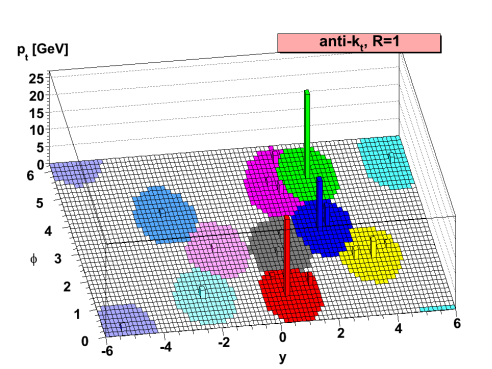
\includegraphics[width=0.5\textwidth]{images/antikt.png}
\caption{Esquema de agrupamiento de topo-clusters realizado por el algoritmo \textit{anti-$k_t$}. \tosolve{Puede que exista una imagen mejor} 
 % \commentNotaIII
 }
  \label{antikt}
\end{figure}

A continuación los jets pasan por una serie de correcciones y calibraciones antes de reconstruir el objeto final para los análisis. Primero se remueve la contribución por pile-up, en el caso de los \textit{large-R} jets afecta principalmente a las distribuciones angulares que son necesarias para la reconstrucción de su masa invariante, y se remueve utilizando una técnica denominada \textit{grooming} descripta en la Referencia \cite{trimming}. Para los \textit{small-R} jets primero se realiza una corrección del origen de su vértice y luego se suprime la contribución por pile-up utilizando métodos que tienen en cuenta la densidad de energía de pile-up \cite{PERF-2016-04} junto con variables asociadas a las trazas y al vértice primario \cite{PERF-2014-03} \tosolve{Tengo que mencionar JVT. JVF tal vez también}.
% \commentred{tengo que mencionar JVT, JVF tal vez también}
A continuación se calibra la energía del jet utilizando simulaciones de MC
\commentyellow{HW: No se si estoy de acuerdo en decir que usan MC. El ultimo paso in situ usa datos... Diría algo como se calibra la energía del jet utilizando MC y datos comparativamente ?. GO: ATL-PHYS-PROC-2017-236: En esta estapa entiendo que se utiliza exclusivamente calibraciónes con MC. Y que posteriormente viene la calibración in situ, que menciono al final del parrafo. No me queda claro del texto si la in situ se usa exclusivamente para datos o si utiliza exclusivamente datos (o ambas)}
. Esto es necesario debido a que gran parte del jet es invisible al detector, por ejemplo cuando el jet se encuentra en las zonas del mismo donde la sensibilidad es baja. 
% Posibilidad de agregar: hadronic showers inherently rely on interactions with the strong force to start electromagnetic cascades, typically via the creation of pi0 and pipm . However, these strong interactions result in a substantial amount of energy going into splitting nuclei, and thus overcoming the binding energy. This energy is not observed
La escala de energía del jet (\textit{Jet Energy Scale}, JES) \cite{JETM-2018-05} calcula un factor de respuesta en bines de $|\eta|$ y \pt utilizando simulaciones de MC, y que al aplicarlo a los datos permite la corrección en energía de los jets. Para los \textit{large-R} jets se aplica a su vez una corrección similar en la masa necesaria para la correcta reconstrucción de su masa invariante. Los \textit{small-R} jets por su parte pasan por una calibración (\textit{Global Sequential Calibration}, GSC) que mejoran la resolución de energía del jet (\textit{Jet Energy Resolution}, JER). Finalmente se realiza una corrección basada en datos y aplicada exclusivamente a los mismos.


% \cite{ATLAS-CONF-2014-018}


% ATL-PHYS-PROC-2017-236
%  Topo-clusters are formed fromseed cell(s) with more than 4σof energy, whereσis the average amount of noise expected in the cellin question, defined as the sum of the expected electronic and pile-up noise [3]. In current data-takingconditions, the pile-up noise dominates over the electronic noise. All cells adjacent to the seed cell(s)in three dimensions are then grouped together, so long as they have at least 2σof energy, and thisprocess repeats until there are no such adjacent cells. The process concludes by adding all calorimetercells adjacent to the topo-cluster, irrespective of their energy.

% topo-clusters can be calibrated at either the raw (electromagnetic, EM) scale, where the energy ofan isolated topo-cluster is the sum of its constituent cell energies, or at the local cell weighting (LCW)scale. The LCW scale accounts for the difference between electromagnetic and hadronic interactionsin the ATLAS calorimeters, thereby correcting the average topo-cluster to the hadronic energy scale.

% l jets in ATLAS make use of standard topo-clusters,  using  EM  topo-clusters  for  small-Rjets  and  LCW  topo-clusters  for  large-Rjets

% topo-clusters are formed, they are naturally pile-up suppressed. However,this form of pile-up suppression is designed for the average topo-cluster in average expected data-taking conditions. By taking advantage of event-by-event measurements of the pile-up levels, as wellas local observables, it is possible to further reduce the pile-up dependence of topo-clusters

%  Two different distance parametersRare typically used, corresponding to differentintended uses.  Jets representing quarks and gluons are typically called small-Rjets, and are recon-structed withR=0.4.  On the other hand, jets representing hadronically decaying massive particlesare typically called large-Rjets, and are reconstructed withR=1.0.

%  In the latter case, the larger radius is useful to capture all of the decay products within a single jet,as the angular separation∆Rbetween the constituents of a massive particleχundergoing a two-bodydecay follow∆R&2mχ/pχT, as seen in Figure 1. For multi-stage decays, such ast→bW→bqq, thedecay products are less collimated, further necessitating the use of large distance parameters.

%  Using large-Rjets is necessary to fully contain the hadronic massive particle decays,  but it comeswith a substantially increased sensitivity to pile-up effects due to the larger fraction of the calorimeterenclosed within the jet volume.  Additionally, while pile-up may be low energy and thus not changethe total jet kinematics by a large amount, it is randomly distributed, and can thus obscure the angularstructure within the jet that is the key to identifying massive particle decays


\subsection{Jets provenientes de quarks bottom ($b$-jets)}

Los decaimientos de los hadrones pesados están gobernados generalmente por el hadrón más pesado en la cascada del decaimiento. Un hadrón $b$ generalmente decae a través de una cascada a un hadrón $c$, que a su vez decae a un hadrón $s$, etc. Esto genera la existencia de múltiples 
\commentyellow{HW: en general es un solo vértice secundario. Te referís acá al algo tipo B- > JPsi ->Ks ?
GO: arXiv:1711.08811: The typical heavy hadron topology presents one or more vertices that are displaced from
the hard-scatter interaction point. The longer lifetimes of heavy-flavor hadrons correspond
to macroscopic decay lengths that can be resolved by the ATLAS vertexing detectors. The
hadrons decay is governed by its heavy quark decay chain. A b-hadron will usually decay
through a cascade to a c-hadron, strange hadron, etc. Therefore, in a b-initiated event, the goal
is to reconstruct not only the primary vertex whence the event initiates, but also a secondary,
and possibly tertiary vertex along the decay cascade. Finally, the heavy-flavor hadrons non-
negligible branching ratio to semi-leptonic decays (21\%) suggests using the presence of soft
muons within jets as yet another discriminating feature for flavor tagging.}
vértices secundarios, que junto con la información de las trazas y la elevada vida media de los hadrones $b$, son utilizados por distintos algoritmos para poder distinguir los hadrones $b$ de hadrones con sabores más livianos (\textit{b-tagging}). Algunos ejemplos de algoritmos \cite{btag} son el MV2 basado en un \textit{boosted decision tree} y compuesto de clasificadores de bajo nivel, y el DL1 basado en una red neuronal profunda. Para cada algoritmo se definen WPs con distintas eficiencias de selección, que a mayor eficiencia mayor es la probabilidad de identificar otros tipos de jets erróneamente como $b$-jets. Con el WP de 77\% del algoritmo MV2 (DL1) 1 de cada 5 (5) $c$-jets, 1 de cada 15 (14) $\tau$-jets y 1 de cada 110 (130) jets livianos son identificados erróneamente como $b$-jets \cite{btag}.

 % The performance of a b-tagging algorithm is characterised by the probability of tagging a b-jet (b-jet tagging efficiency,εb) and the probability of mistakenly identifying a c-jet or a light-flavour jet as a b-jet, labelled εc (εl). In this paper, the performance of the algorithms is quantified in terms of c-jet and light-flavour jet rejections, defined as 1/ε cand 1/εl, respectively


\section{Energía transversa faltante}\label{sec:met}


El momento transverso faltante es una variable que se utiliza como análogo al momento de las partículas que prácticamente no interactúan con el detector, por ejemplo neutrinos o partículas más allá del SM, ya que este último naturalmente no puede ser medido por ninguno de los subdetectores. El momento en la dirección del haz que acarrea cada partón previo a la colisión es desconocido, pero en la dirección transversa al haz se puede considerar que es nulo. Por conservación del momento se puede deducir que luego de la colisión la suma de los momentos en el plano transverso de todas las partículas producidas debería ser nulo, y en caso de no serlo puede ser un indicio de una partícula que escapó la detección. La reconstrucción del momento transverso faltante se basa en esta conservación y se define como menos la suma de los momentos transversos de todas las partículas observadas en el evento. En esta suma se incluyen los electrones, muones, fotones, taus decayendo hadrónicamente y jets reconstruidos con los métodos descriptos en las secciones anteriores. Además se incluye un termino (\textit{soft}) que tiene en cuenta el momento en la traza de las partículas que dejaron señal en el ID pero que no llegaron a reconstruirse. Quedando la definición del vector momento transverso faltante como \cite{PERF-2016-07}:

\begin{equation}
\textbf{E}_{\text{T}}^{\text{miss}} = -\sum_{i}\textbf{p}_{\text{T}}^{e_i}-\sum_{i}\textbf{p}_{\text{T}}^{\gamma_i}-\sum_{i}\textbf{p}_{\text{T}}^{\tau_i}-\sum_{i}\textbf{p}_{\text{T}}^{j_i}-\sum_{i}\textbf{p}_{\text{T}}^{\mu_i}-\sum_{i}\textbf{p}_{\text{T}}^{\text{Soft}_i}
\end{equation}


En general no se utilizan las componentes de este vector sino que se utiliza su módulo (\met) y su ángulo ($\phi^{\text{miss}}$), y cuando se menciona al momento transverso faltante se está haciendo referencia a su módulo. Cabe aclarar que esta definición introduce un sesgo a tener \met no nula en eventos donde no se produjo ninguna partícula no interactuante, debido a la incorrecta o insuficiente reconstrucción de todos los objetos presentes en el evento. Otra variable que se utiliza además es $\Sigma E_{\text{T}}$ que se define como la suma del módulo de los momentos de todas las partículas anteriormente consideradas. 
% \commentHW{hace falta esto ? no lo usamos ?} \commentgreen{Se usa para MET significance, en caso de no usar esta variable en el análisis lo podríamos sacar}

Como la reconstrucción se realiza de forma independiente para cada objeto, puede ocurrir que dos objetos distintos compartan algunas celdas calorimétricas. Para evitar el doble conteo, se define el siguiente orden de prioridad: electrones, fotones, taus y jets \cite{PERF-2011-07, PERF-2014-04}. Si alguna de estas partículas comparte celdas con otra de una prioridad mayor, la misma se elimina del cálculo de \met. Los muones son principalmente reconstruidos en el ID y el MS, por lo que el solapamiento con las demás partículas es mínimo y salvo algunos casos particulares ninguno es descartado. Muones no aislados que se solapan con los jets, jets que se solapan mínimamente con otros objetos o jets reconstruidos a partir de un depósito de energía de muones o de pile-up tienen un tratamiento especial descripto en la Referencia \cite{PERF-2016-07}. En el término \textit{Soft} se incluyen solamente aquellas trazas provenientes del vértice principal que no estén asociadas las partículas anteriormente seleccionadas. Los depósitos de partículas neutras \textit{soft} no se incluyen en este término ya que en su mayoría son producto del pileup y su inclusión reduce el desempeño en la reconstrucción de \met.


% \pdfmarkupcomment[markup=StrikeOut,color=red]{Los objetos que se incluyen en el cálculo de MET dependen de la selección de cada análisis, en el caso del presente análisis la selección base utilizada está descripta en la Sección}{Al final esto estaba mal, MET se obtiene independiente de nuestra seleccion baseline. Podría sacar esto y capaz unificar lo de soft con el parrafo anterior.}
% \commentHW{no esta repetido esto del término soft ?}
% \commentgreen{Decis por el primer párrafo? Como que ahí lo introduje y acá pongo algunos detalles más, que tampoco son muchos...}


